% Some commands used in this file
\newcommand{\package}{\emph}

\setcounter{chapter}{-1}
\chapter{Instruction Manual}

\section{Environment}

\begin{figure}[h]
\centering
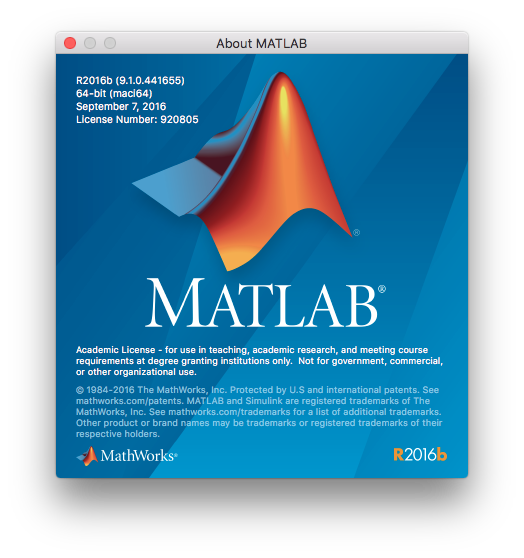
\includegraphics[width=0.6\textwidth]{aboutMatlab.png}
\caption{MATLAB Version Information (MATLAB for MAC OS X)}
\end{figure}

The code is written in Mathworks \textbf{\copyright MATLAB}. Due to the differences in several matrix operation, the code only works properly in \textbf{R2016b} version. Operating Systems of testing environments are \textbf{Linux Ubuntu 14.04 LTS} and \textbf{Apple Mac OS X El Capitan Version 10.11.6.}

We did not use any external libraries but only the modules developed during the exercises sessions and several MATLAB classes or functions which are allowed. (e.g. \textit{vision.PointTracker})

\section{Files}
\subsection*{Scripts}

.m script files are under \textit{src} directory. 

\begin{itemize}
\item \textit{main.m} \quad A main script for visual odometry pipeline. It invokes VO functions such as \textit{initializeVO, processFrame, bundleAdjustment} and \textit{visualizeFrame.} Also, it includes several running options such as choosing data set among KITTI / Malaga / Parking / Seoul and turn on/off features etc.

\item \textit{create\_bag.m} \quad This script generates bag of visual words and image index for each data set which can be used for image retrieve test and debug. Since place recognition does not work properly in our pipe line, it is deprecated now.
\end{itemize}

\subsection*{Visual Odometry Functions}

.m files below includes core logic of our VO pipeline. Please refer to \textbf{Monocular Visual Odometry} section for more details. Files are under \textit{src/visual\_odometry} directory.

\begin{itemize}
\item \textit{initializeVO.m} \quad Function for VO initialization operation.  
\item \textit{processFrame.m} \quad Function for VO continuous operation.
\item \textit{bundleAdjustment.m} \quad Function for bundle adjustment.
\item \textit{getParams.m} \quad This functions returns proper parameters for each data sets which were carefully chosen.
\item Functions for Loop Closure (\textit{./loopClosure\_sub}) 
\item Other sub-functions for functions above (\textit{./other\_sub})
\end{itemize}

\subsection*{Classes}

Class files are written in Object Oriented Programming style for containing data such as state, landmarks, candidates and parameter(\textit{Params\_XXX.m} files) They also includes several methods to process these data. Files are under \textit{src/class} directory.\newline \newline
Note: Please do not change value of parameter class properties. These values have been carefully chosen. 

\subsection*{Package Functions}

These .m files are developed during the exercise session. The files are under \textit{src/exercise\_packages} directory.

\subsection*{Files for Debugging}

These .mat files were used for debugging. It includes exported bag of visual words, image index etc. The files are under \textit{src/var\_debug} directory. \newline 
Note: For test VO, you do not need to concern about these files.

\subsection*{Data Set Files}

Data set files are images for VO pipeline. The files are under \textit{data} directory. \textbf{For submitted version, we included whole dataset files in the directory.} Please refer to \textbf{Installation and Running} section.

\begin{itemize}
\item KITTI \quad Path of the data set is \textit{data/kitti}  
\item Malaga \quad Path of the data set is \textit{data/malaga-urban-dataset-extract-07} 
\item Parking \quad Path of the data set is \textit{data/parking} 
\item Seoul \quad Data set which was created by us. It was generated from video recorded by iPhone 6 and processed (i.e. calibrated and rectified) using \href{https://www.vision.caltech.edu/bouguetj/calib_doc/}{MATLAB Camera Calibration Toolbox for MATLAB by Caltech.} Path of the data set is \textit{data/iphone} 
\end{itemize}



\section{Installation and Running}

We submit one .zip file which contains whole code and our own dataset. For a testing, extract the .zip file and please set dataset paths first, which defined in main script. Finally run \textit{main.m} script. \textit{main.m} automatically refer to other dependencies for running VO pipeline. 

Remark, our VO pipeline only works in \textbf{MATLAB R2016b} 

Note: Before run main script, \textbf{please check if you are in the \textit{src} directory.} In only works properly when work directory is \textit{src} directory. 

